% Written by tekx 0.2.0 from everything.tekx.
\documentclass[a4paper]{amsart}
\usepackage[T1]{fontenc}
\usepackage{amssymb}
\usepackage{mathrsfs}
\usepackage{graphicx}
\usepackage[hidelinks]{hyperref}

\makeatletter
\@ifundefined{KV@Gin@alt}{\define@key{Gin}{alt}{}}{}
\makeatother

\theoremstyle{plain}
\newtheorem{theorem}{Theorem}[section]
\newtheorem{lemma}[theorem]{Lemma}
\newtheorem*{theorem*}{Theorem}
\newtheorem{postulate}[theorem]{Postulate}

\numberwithin{equation}{section}
\DeclareMathOperator{\Var}{Var}

\title[Everything]{Everything at Once}
\author{Ada Lovelace}
\email{ada@example.org}
\address{University of London}
\author{Charles Babbage}
\address{Cambridge}
\date{\today}
\subjclass[2020]{11N36 (primary)}
\keywords{integration, consistency}

\begin{document}

\begin{abstract}
We test that every part of tekx agrees with every other \cite{hooley}, \cite[p. 3]{landau}.

\end{abstract}

\maketitle

\tableofcontents

\section{Introduction}\label{intro}

Work at the Analytical Engine Laboratory showed\footnote{A footnote with $x^{2}$ and a citation \cite{vallee}.} that

\begin{equation}\label{gauss}
  \int_{-\infty}^{\infty} e^{-x^{2}} \, \mathrm{d} x = \sqrt{\pi}
\end{equation}

and, by Theorem~\ref{main} and \eqref{gauss}, the variance $\operatorname{Var} X$ and $\lVert 2 \rVert (v)$ behave.

\begin{theorem}[Main]\label{main}
For every $n \geq 1$, $\sum_{k = 1}^{n} k = (n(n + 1))/2$.

\end{theorem}

\begin{proof}
Induction on $n$.

\end{proof}

\begin{lemma}\label{lem}
The long identity

\begin{equation}\label{binom4}
  (a + b)^{4} = (a + b)^{2} (a + b)^{2} = (a^{2} + 2 a b + b^{2}) (a^{2} + 2 a b + b^{2}) = a^{4} + 4 a^{3} b + 6 a^{2} b^{2} + 4 a b^{3} + b^{4}
\end{equation}

holds.

\end{lemma}

\begin{theorem*}[Unnumbered]
An unnumbered statement, cited by Lemmas \ref{lem} and \ref{main2}.

\end{theorem*}

\begin{postulate}\label{post}
Every integral converges.

\end{postulate}

\section{Structure}\label{structure}

\begin{itemize}
\item a bullet with $\alpha$
\item 
another

\begin{enumerate}
\item nested
\item numbered
\end{enumerate}

\end{itemize}

\begin{center}
\begin{tabular}{cl}
\hline
\textbf{Symbol} & \textbf{Meaning} \\
\hline
$\mathbb{N}$ & natural numbers \\
$\mathbb{R}$ & real numbers \\
\hline
\end{tabular}
\end{center}

\begin{figure}[htbp]
\centering
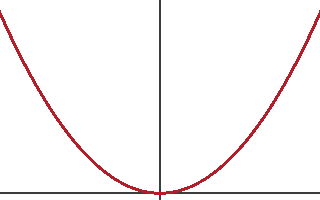
\includegraphics[width=0.4\linewidth,alt={The parabola y equals x squared.}]{parabola.png}
\caption{The graph of $y = x^{2}$.}\label{fig}
\end{figure}

See Figure~\ref{fig} and Section~\ref{structure}, and \cite{erdos,thesis,arxiv}.

\begin{theorem}\label{main2}
A second theorem: $\lvert x \rvert = \begin{cases} x \text{ if } x \geq 0 & -x \text{ otherwise } \end{cases}$.

\end{theorem}

\appendix

\section{Tables of values}\label{app}

\begin{lemma}\label{applem}
In Appendix~\ref{app}, Lemma~\ref{applem} holds:

\begin{equation}\label{bound}
  g(x) \leq 2 x^{1/4}
\end{equation}

\end{lemma}

\bibliographystyle{amsplain}
\bibliography{refs}

\end{document}
